\documentclass[aspectratio=169,xcolor=dvipsnames,14pt]{beamer}
\usepackage{graphicx}
\usepackage{siunitx}
\usepackage{amssymb}

\setbeamertemplate{itemize item}[circle]
\title{Kernfusion}
\author{\color{LightGrey}Jan Kunde}
\date{}
\usefonttheme{serif}
\definecolor{LightGrey}{rgb}{242, 242, 242}
\usecolortheme[named = LightGrey]{structure}
\beamertemplatenavigationsymbolsempty
%Global Background must be put in preamble
\usebackgroundtemplate%
{%
    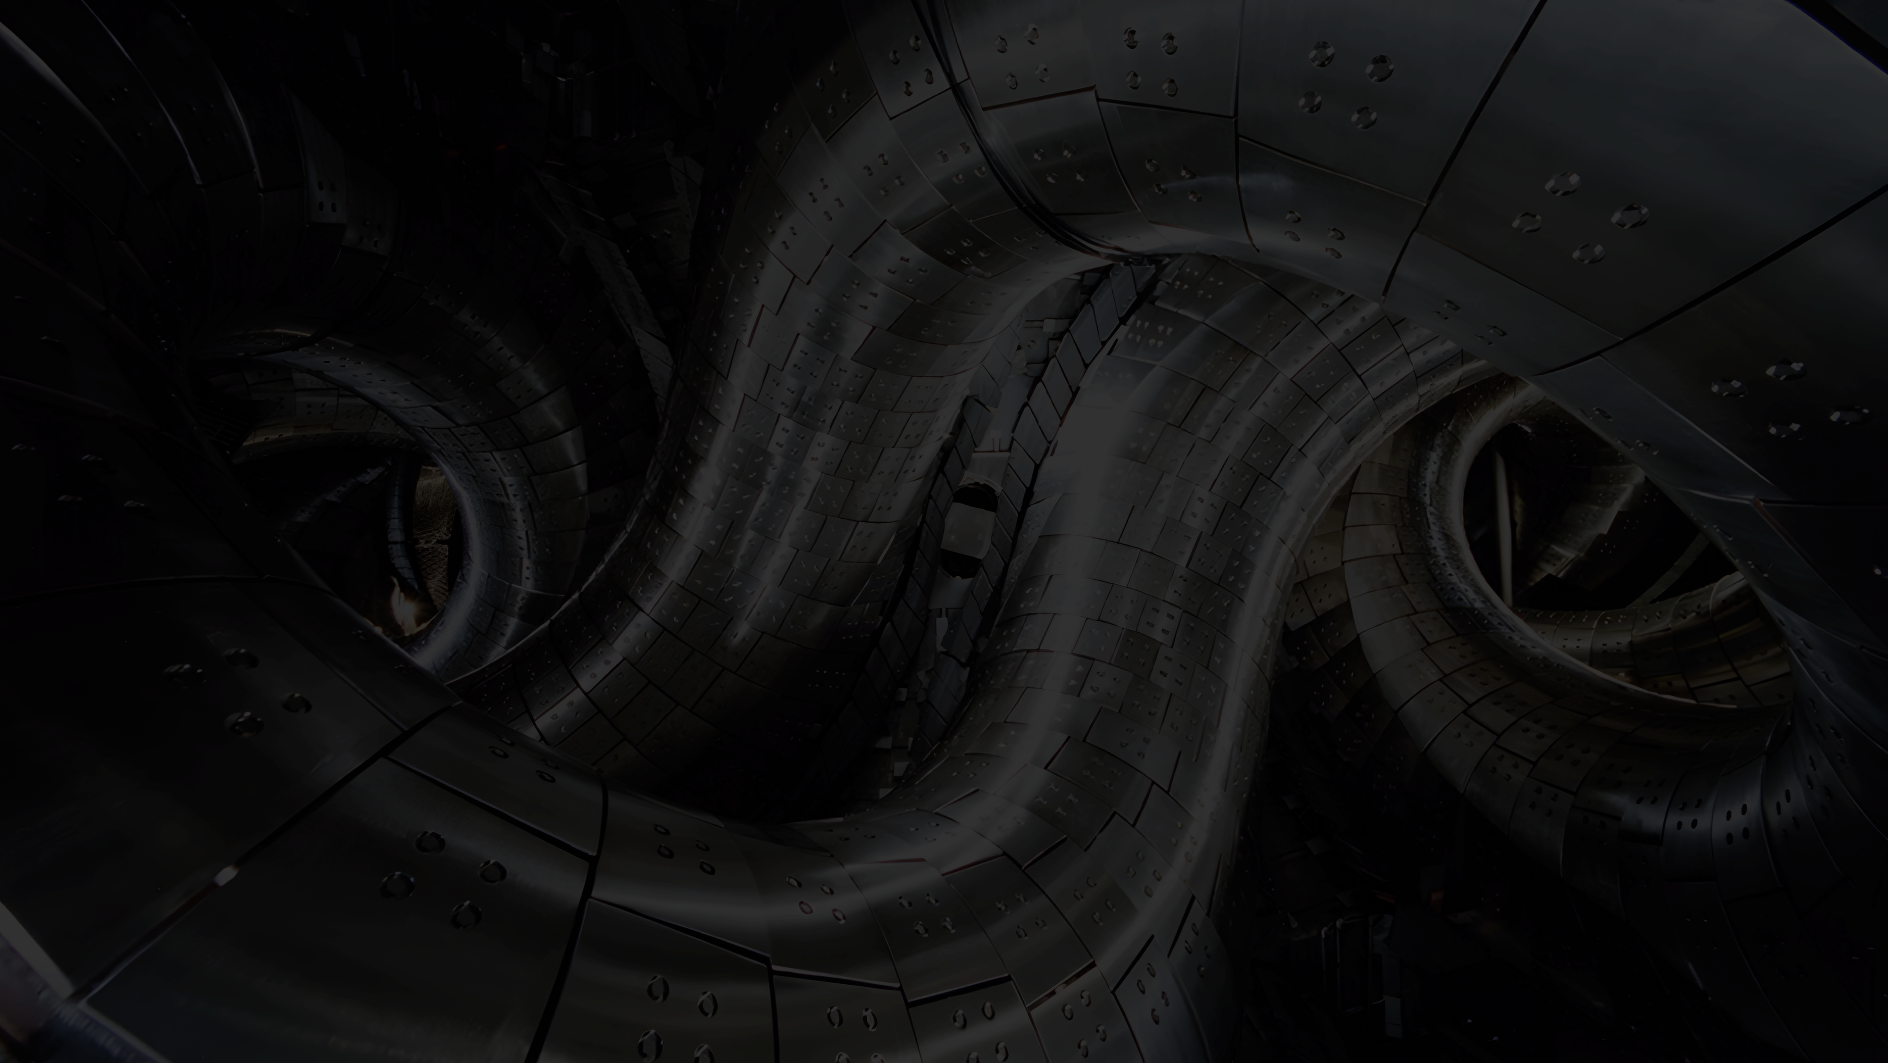
\includegraphics[width=\paperwidth,height=\paperheight]{background.png}%
}



\begin{document}
\color{LightGrey}
\begin{frame}{}
\color{LightGrey}
\maketitle
\end{frame}


% Inhalt
{
\begin{frame}{Inhalt}
\begin{itemize}
    \color{LightGrey}
\item Grundlagen der Kernfusion
\item Geschichte der Kernfusion
\item Stellare Kernfusion
\item Kernfusion zur Energiegewinnung
\end{itemize}
\end{frame}
}

% Grundlagen der Kernfusion
{
\begin{frame}{Grundlagen der Kernfusion}
\begin{itemize}
    \color{LightGrey}
\item Verschmelzen von Atomkernen
\item Kerne müssen Coulombbarriere überwinden / durchtunneln   
\item Sowohl exotherme als auch endotherme Fusionsreaktionen
\item Exothermität / Endothermität durch Massendefekt zu erklären
\end{itemize}
\end{frame}
}

%Geschichte der Kernfusion
{
\begin{frame}{Geschichte der Kernfusion}
\begin{itemize}
    \color{LightGrey}
\item 1917, Lange vor Kernspaltung entdeckt
\item 1920 als Energiequelle von Sternen erkannt
\item 1952/53 erste auf Fusion bassierende Wasserstoffbombe
\item Seit Entwicklung der Fissions-Bombe Forschung an wirtschaftlicher Nutzung
\end{itemize}
\end{frame}
}

%Stellare Kernfusion
{
\begin{frame}{Stellare Kernfusion}
    \begin{itemize}
        \color{LightGrey}
        \item Kleinere Sterne - Proton-Proton-Reaktion
        \item Größere Sterne - Bethe-Weizsäcker-Zyklus
        \item Entstehung von Kernen bis $A = 60-70$
    \end{itemize}
\end{frame}
}

    %Proton-Proton-Reaktion
    {
    \begin{frame}{Proton-Proton-Reaktion}
        \begin{columns}
            \begin{column}{0.7\textwidth}
                \begin{itemize}
                    \color{LightGrey}
                    \item Startreaktion: \\ \begin{math} {\displaystyle \mathrm {{}^{2}H+{}^{1}H\to {}^{3}He+\gamma +5{,}493\;MeV} }    \end{math}
                    \item Folgereaktion: \\ \begin{math}  {\displaystyle \mathrm {{}^{3}He+{}^{3}He\to {}^{4}He+2\,{}^{1}H+12{,}86\;MeV} }    \end{math}
                    


                \end{itemize}
            \end{column}

            \begin{column}{0.3\textwidth}
                \begin{itemize}
                    \color{LightGrey}
                    \item Hauptreaktion der Sonne
                    \item ca. \num{1.4e10} Jahre bis Start reaktion pro Proton
                    \item + \num{26.196} MeV
                \end{itemize}
            \end{column}
        \end{columns}
        

    \end{frame}
    }

    %Bethe-Weizsäcker-Zyklus
    {
    \begin{frame}{Bethe-Weizsäcker-Zyklus}
        \begin{columns}
            
            \begin{column}{0.7\textwidth}
                \begin{itemize}
                    \color{LightGrey}
                    \item
                    \begin{math}
                        {\displaystyle \mathrm {_{\ 6}^{12}C+_{1}^{1}H\to _{\ 7}^{13}N+\gamma+1,96 \ MeV}}
                    \end{math}

                    \item 
                    \begin{math}
                        {\displaystyle \mathrm {_{\ 7}^{13}N \to _{\ 6}^{13}C+ {e}^{+} + \nu_{e}+1,37 \ MeV }}
                    \end{math}

                    \item \begin{math}
                        {\displaystyle \mathrm {_{\ 7}^{13}N \to _{\ 6}^{13}C+ {e}^{+} + \nu_{e}+1,37 \ MeV }}
                    \end{math}

                    \item
                    \begin{math}
                        {\displaystyle \mathrm {_{\ 6}^{12}C+_{1}^{1}H\to _{\ 7}^{14}N+\gamma+7,54 \ MeV}}
                    \end{math}

                    \item
                    \begin{math}
                        {\displaystyle \mathrm {_{\ 7}^{14}N+_{1}^{1}H\to _{\ 8}^{15}N+\gamma+7,35 \ MeV}}
                    \end{math}

                    \item
                    \begin{math}
                        {\displaystyle \mathrm {_{\ 8}^{15}O \to _{\ 7}^{15}N+{e}^{+} + \nu_{e}+1,73 \ MeV}}
                    \end{math}

                    \item
                    \begin{math}
                        {\displaystyle \mathrm {_{\ 7}^{15}N+_{1}^{1}H \to _{\ 6}^{12}C+_{2}^{4}He+4,96 \ MeV}}
                    \end{math}
                \end{itemize}
            \end{column}

            \begin{column}{0.3\textwidth}
                \begin{itemize}
                    \color{LightGrey}
                    \item \begin{math} M > M_{Sonne} \end{math} für sig. Effekt auf Energiebilianz
                    \item Ab \num{14e6}$^{\circ}$ Kelvin
                    \item +\num{25.03} MeV
                    \item \num{1.193} MeV weniger als P-P-Reaktion
                \end{itemize}
            \end{column}
        \end{columns}
    \end{frame}
    }

%Kernfusion zur Energiegewinning
\begin{frame}{Kernfusion zur Energiegewinning}
    \begin{columns}
        \begin{column}{0.5\textwidth}
            \begin{figure}
                \centering
                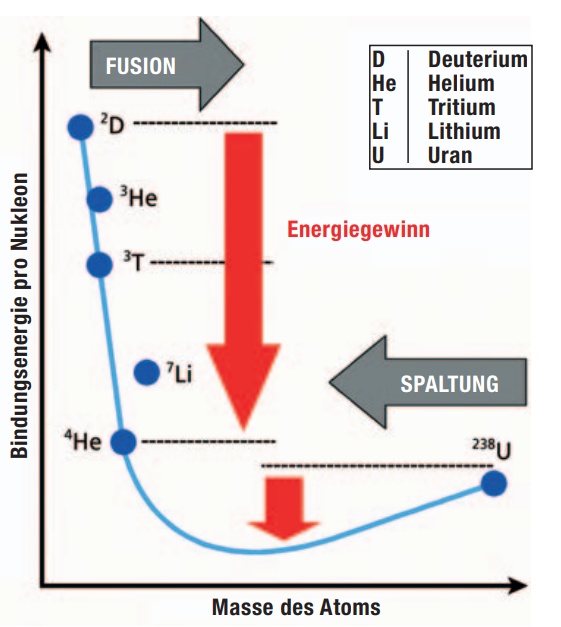
\includegraphics[width=0.7\textwidth]{Bindungsenergie.png}
            \end{figure}
        \end{column}

        \begin{column}{0.5\textwidth}
            \begin{figure}
                \centering
                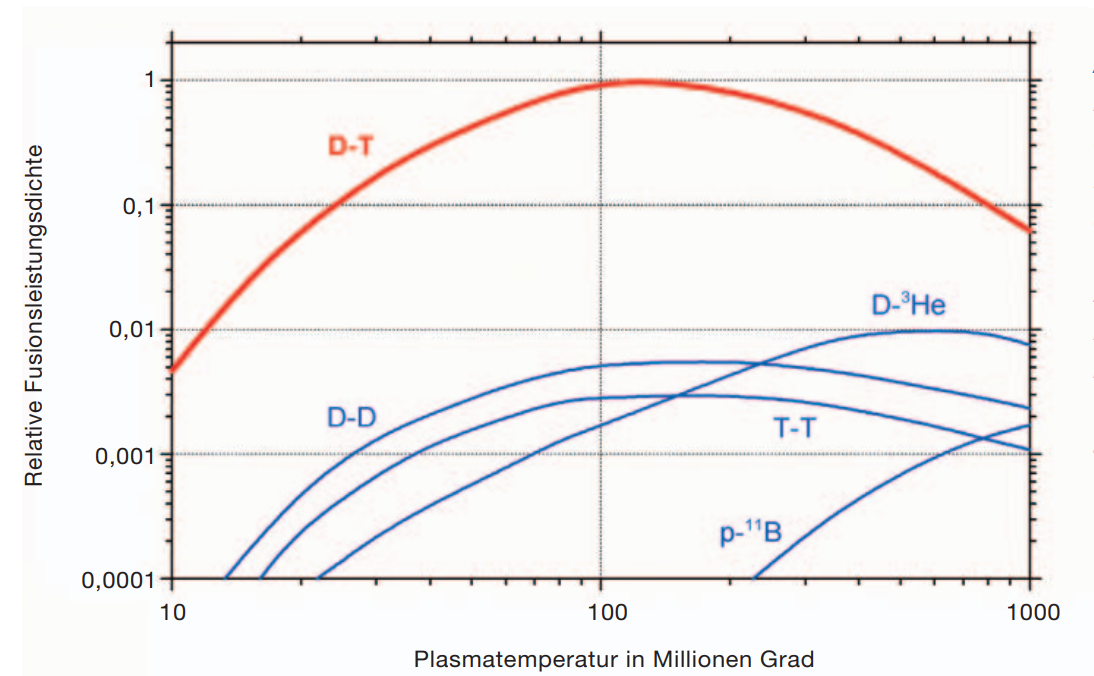
\includegraphics[width=1\textwidth]{Fusionsleistungsdichte.png}
            \end{figure}
        \end{column}
    \end{columns}
\end{frame}
    
    %Deuterium-Tritium-Reaktion
    \begin{frame}{Deuterium-Tritium-Reakion}
        \begin{columns}
            
            \begin{column}{0.7\textwidth}
                
            \end{column}

            \begin{column}{0.3\textwidth}
                \begin{itemize}
                \color{LightGrey}
                    \item Lawson-Kriterium muss erfüllt sein $(T\cdot\rho\cdot\tau _{E})$
                    \item $T = 150\cdot{10}^{6}$ Kelvin
                    \item $\rho \ll \rho_{Sonne}$
                \end{itemize}
            \end{column}

        \end{columns}
    \end{frame}
    %Weitere Denkbare Reakionen
    %Tokamak-Architektur
    %Stellerator-Architektur

%Quellen	
\begin{frame}{Quellen}
\begin{itemize}
    \color{LightGrey}
\item https://www.fusion.kit.edu/downloads/Kernfusion.pdf
\item https://de.wikipedia.org/wiki/Kernfusion
\item https://www.fraunhofer.de
\end{itemize}
\end{frame}

\end{document}